% !TeX spellcheck = <none>
%\documentclass[brudnopis]{xmgr}
% Jeśli nowe rozdziały mają się zaczynać na stronach
% nieparzystych:
\documentclass[openright]{xmgr}

% install minted package to highlight source code
\usepackage{minted}

\usepackage{epigraph}
\usepackage{url}
\usepackage{hyperref}
\def\UrlBreaks{\do\/\do-}
\usepackage{float}

\defaultfontfeatures{Scale=MatchLowercase}
\setmainfont[Numbers=OldStyle,Ligatures=TeX]{Minion Pro}
\setsansfont[Numbers=OldStyle,Ligatures=TeX]{Myriad Pro}
% for fontspec version < 2.0
%\setmainfont[Numbers=OldStyle,Mapping=tex-text]{Minion Pro}
%\setsansfont[Numbers=OldStyle,Mapping=tex-text]{Myriad Pro}
%\setmonofont[Scale=0.75]{Monaco}

% Opcjonalnie identyfikator dokumentu
% drukowany tylko z włączoną opcją 'brudnopis':
\wersja   {wersja wstępna [\ymdtoday]}

\author   {Piotr Lewandowski}
\nralbumu {215575}
\email    {poczta@piotrl.net}

\title    {Analiza wpływu nawyków muzycznych na aktywności wykonywane przy komputerze}
\date     {2017}
\miejsce  {Gdańsk}

\opiekun  {dr W. Bzyl}

% dodatkowe polecenia
%\renewcommand{\filename}[1]{\texttt{#1}}
%\definecolor{stress}{cmyk}{0,1,0.13,0} % RubineRed
%\definecolor{topic}{cmyk}{0.98,0.13,0,0.43} % MidnightBlue

\begin{document}

% streszczenie
\begin{abstract}
    W ramach pracy magisterskiej napisano aplikację internetową,
    wdrożoną na chmurze Digital Ocean pod adresem \url{http://tbd.digitalocean.com/}
    z przygotowanymi danymi testowymi pod kontem (user: test, password: test).

    Aplikacja umożliwia import danych użytkownika z dwóch serwisów,
    RescueTime — lista aktywności oraz
    Last.fm — lista odsłuchiwanych utworów.
    Pobrane dane są połączone na wspólnej osi czasu i wizualizowane pod różnymi względami za pomocą wykresów oraz tabel.

    Mechanizm agregacji napisany jest w języku Java i frameworku Spring,
    dane przechowywane są w bazie danych PostgreSQL,
    a warstwa wizualna została stworzona w frameworku Material Design oraz JavaScript,
    do generowania wykresów użytko biblioteki Google Charts.

    Kod znajduje się w prywatnym repozytorium GIT (pod adresem \url{https://github.com/piotrl/master-thesis}),
    pytania o dostęp lub o pracę można kierować na mail: \url{mail@piotrl.net}.
\end{abstract}

% słowa kluczowe
\keywords{
    Aggregation,
    Data Integration,
    Visualisation,
    PostgreSQL,
    JavaScript,
    Java
}

% tytuł i spis treści
\maketitle

% wstęp
\introduction

\epigraph{Without deviation from the norm, progress is not possible}{\textit{Frank Zappa}}

    Właśnie słucham playlisty
    \footnote{Playlista ``Writing --- Instrumental Hip-Hop'' jest dostępna na Spotify.
    \url{https://open.spotify.com/user/exmortisinvictus/playlist/69GtfS8diB8bUHQ74V4yuP}}
    z muzyką która pomaga mi się skupić podczas pisania tego wstępu.
    Gdy programuję, zwykle słucham muzyki innej niż podczas pisania ---
    w pracy, by się odciąć od zewnętrznych dźwięków, a w domu, by się odpowiednio nastroić.
    Gdy mam trudny problem do rozwiązania to preferuję absolutną ciszę.

    Podobnie jak ponad 36 tysięcy innych programistów odpowiadających na pytania w corocznej ankiecie StackOverflow \cite{stackoverflow:survey2017}.
    W pytaniu ``Ideal Auditory Environment for Coding''
    więszkość badanych słucha muzyki, duży odsetek preferuje skrajną ciszę w pracy, natomiast niewielu preferuje rozpraszacze w tle:
    \begin{itemize}
        \item 59.6\% -- Turn on some music
        \item 24.2\% -- Keep the room absolutely quiet
        \item 7.1\% -- Put on some ambient sounds (e.g. whale songs, forest sounds)
        \item 3.5\% -- Something else
        \item 3.2\% -- Put on a movie or TV show
        \item 2.3\% -- Turn on the news or talk radio
    \end{itemize}

    Will Henshall na konferencji TEDx \cite{tedx:music-at-work} stwierdza, że m.in. muzyka klasyczna i Elektro pozytywnie sprzyjają na skupienie,
    natomiast instrumenty brzmiące jak ludzki głos, wokal i elektryczna gitara rozpraszają naszą uwagę.
    Wideo obejrzano ponad 400 tysięcy razy, a sama koncepcja została rozwinięta w projekcie Focus@Will
    \footnote{Focus@Will --- serwis sugerujący szereg playlist pomagający zwiększyć produktywność. \url{https://en.wikipedia.org/wiki/Focus@Will}}.

    Próbuję zweryfikować te założenia przez stworzenie aplikacji, która analizuje moje własne aktywności i muzykę, którą słucham.
    Jednym z mierników, którym się posługuję jest ``Attention Span''
    \footnote{Attention Span --- moment w którym jesteśmy maksymalnie skoncentrowani,
    często nazywane flow. \url{https://en.wikipedia.org/wiki/Attention_span}}.
    Dla uproszczenia tego projektu, przyjmuję założenie, że ``Attention Span'' to czas od początku rozpoczęcia zadania do momentu zmiany aktywnego okna.

    Celem pracy jest opis pełnego procesu budowy aplikacji opartej o analizę danych wraz z ich interpretacją i wizualizacją.

    Opis zaczynam od mechanizmu importu danych z zewnętrznych źródeł, w którym charakteryzuję sposób komunikacji z dostawcami API
    oraz definiuję problemy, którym należy stawić czoła przy budowie agregatora danych.

    W drugim rozdziale przeprowadzam analizę zebranych danych, zaczynając od zapoznania specyfiki struktury danych w bazie
    oraz przeprowadzenia ogólnej statystki, by zobrazować skalę, po której się poruszam.
    Opisałem, w jaki sposób przeprowadzam korektę w przypadku duplikatów, niepełnych lub błędnych danych.

    Rozdział trzeci zawiera przedstawienie zwizualizowanych efektów analizy w postaci wykresów i screenshotów z aplikacji.
    Definiowaniuję sposób budowania zapytań SQL, by zwracały odpowiednio uszeregowane dane w czasie z wybranym interwałem.

    Rozdział czwarty poświęcam architekturze projektu, użytych narzędzi oraz instrukcję uruchomienia projektu lokalnie lub na serwerze.

    Rysunki i tabele są opracowania własnego, chyba że oznaczyłem inaczej.

\chapter{Import danych}

    \section{Wybór dostawców danych}

    Podstawą działania aplikacji są dane z komputera użytkownika,
    lista aktywności wykonywanych oraz odsłuchiwana muzyka w tym samym czasie.
    Aby zdobyć te dane, należałoby napisać program śledzący aktywne procesy i logujący każdą zmianę na serwer.
    Potrzebny byłby też plugin do odtwarzacza muzycznego który na podstawie tagów ID3 plików logował aktualnie słuchaną piosenkę.
    Zdecydowałem się jednak skorzystać z istniejących rozwiązań, z których użytkownicy mojej aplikacji mogliby również korzystać.

    Podstawowym wymaganiem jest to, by serwisy były już dłuższy czas na rynku oraz udostępniały archiwalne dane za pomocą publicznego API.
    Dzięki temu nie ma potrzeby oczekiwania na zbudowanie zbioru danych do po rejestracji nowego użytkowniku,
    od razu można rozpocząć analizę ze zbiorem przygotowanym przed rejestracją.

    Wybrałem dwa dobrze mi znane serwisy --- RescueTime oraz Last.fm,
    oba są popularne w swojej klasie oraz dostarczają publiczne API dla danych użytkownika.

        \section*{RescueTime}

        \begin{figure}
          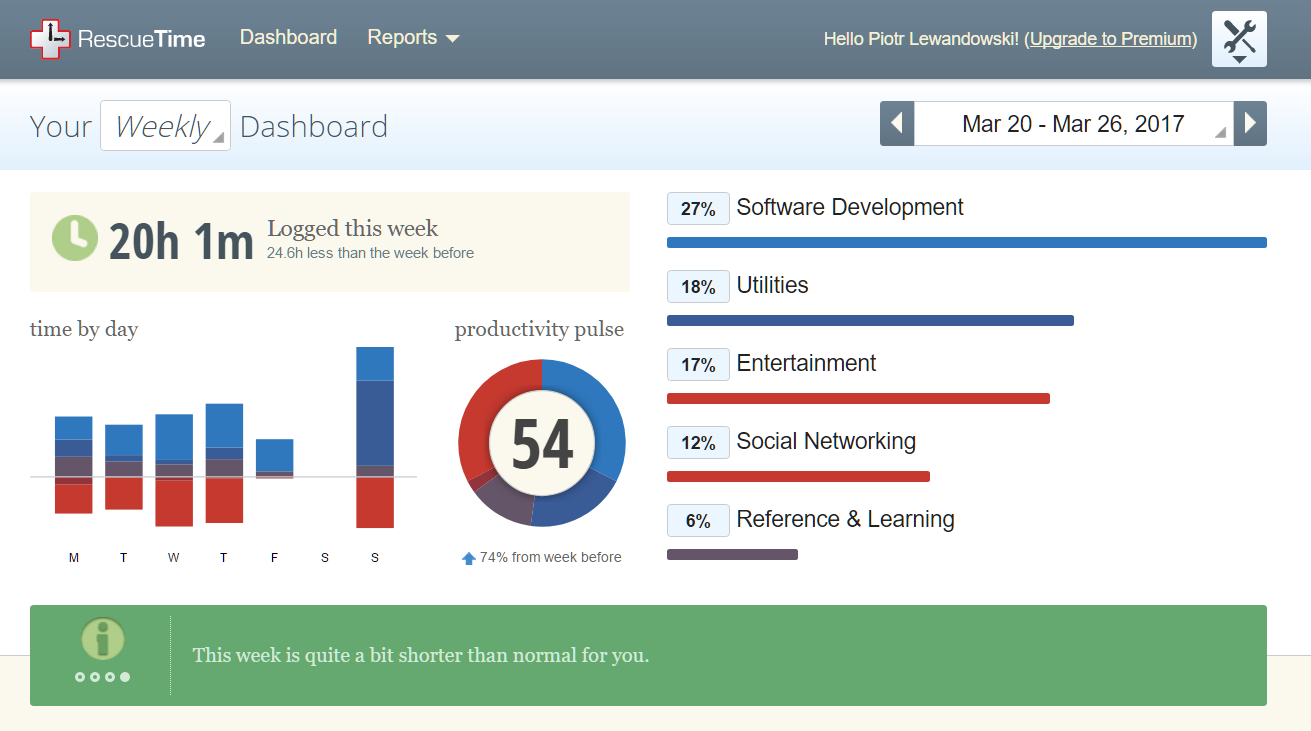
\includegraphics[width=\linewidth]{fig/rescuetime-dashboard.png}
          \caption{Tygodniowy raport aktywności RescueTime}
          \label{fig:rescuetime-dashboard}
        \end{figure}

            RescueTime to program, który loguje aktualnie otwarte i aktywne okno
            i wysyła te dane do serwisu internetowego RescueTime.com.
            Podstawową cechą tego serwisu jest automatyczne kategoryzowanie aktywności oraz ustawienie produktywności w 5 punktowej skali:
            „Bardzo produktywny”, „Produktywny”, „Neutralny”, „Rozpraszający” i „Bardzo rozpraszający”.

            Serwis uczy się dopasowywać aktywności do kategorii na podstawie wcześniejszych oznaczeń użytkowników.
            Dla przykładu odtwarzacz wideo VLC jest przypisany do kategorii „Entertainment” ze statusem „Bardzo rozpraszający”,
            natomiast przeglądanie plików programem Windows Explorer jest w kategorii „Utilities” ze statusem „Neutralny”.

            Dzięki temu jesteśmy w stanie obliczyć nasz codzienny współczynnik produktywności,
            sumując czas spędzony na aktywnościach z każdej kategorii.

            \begin{table}[]
            \centering
            \begin{tabular}{lll}
                \hline
                \multicolumn{1}{l|}{Aktywność} & \multicolumn{1}{l|}{Kategoria} & Produktywność \\ \hline
                idea64                         & Software Development           & +2            \\
                NotePad++                      & Software Development           & +2            \\
                postgresql.org                 & Reference \& Learning          & 0             \\
                twitter.com                    & Social Networking              & -1            \\
                analytics.twitter.com          & Social Networking              & -2            \\
                youtube.com                    & Entertainment                  & -2            \\
                outlook.office.com             & Communication \& Scheduling    & 0             \\
                wunderlist                     & Business                       & +2
                \end{tabular}
                \caption{
                    Lista przykładowych aktywności wraz z ich kategoriami. Skala produktywności od +2 do -2
                }
                \label{RescueTime --- lista przykładowych aktywności}
            \end{table}

            Program jest w stanie rozpoznać nie tylko tytuły aktualnie otwartych okien,
            ale również w przypadku przeglądarki – adresy odwiedzanych stron internetowych,
            jest to bardzo ważne ze względu na dominującą ilość czasu spędzonego w samej przeglądarce.

            Dostęp do informacji użytkownika odbywa się za pomocą REST API z tokenem uwierzytelniającym.
            W przypadku darmowego konta mamy dostęp do danych sprzed 3 miesięcy w formacie JSON.

        \section*{Last.fm}

            \begin{figure}
                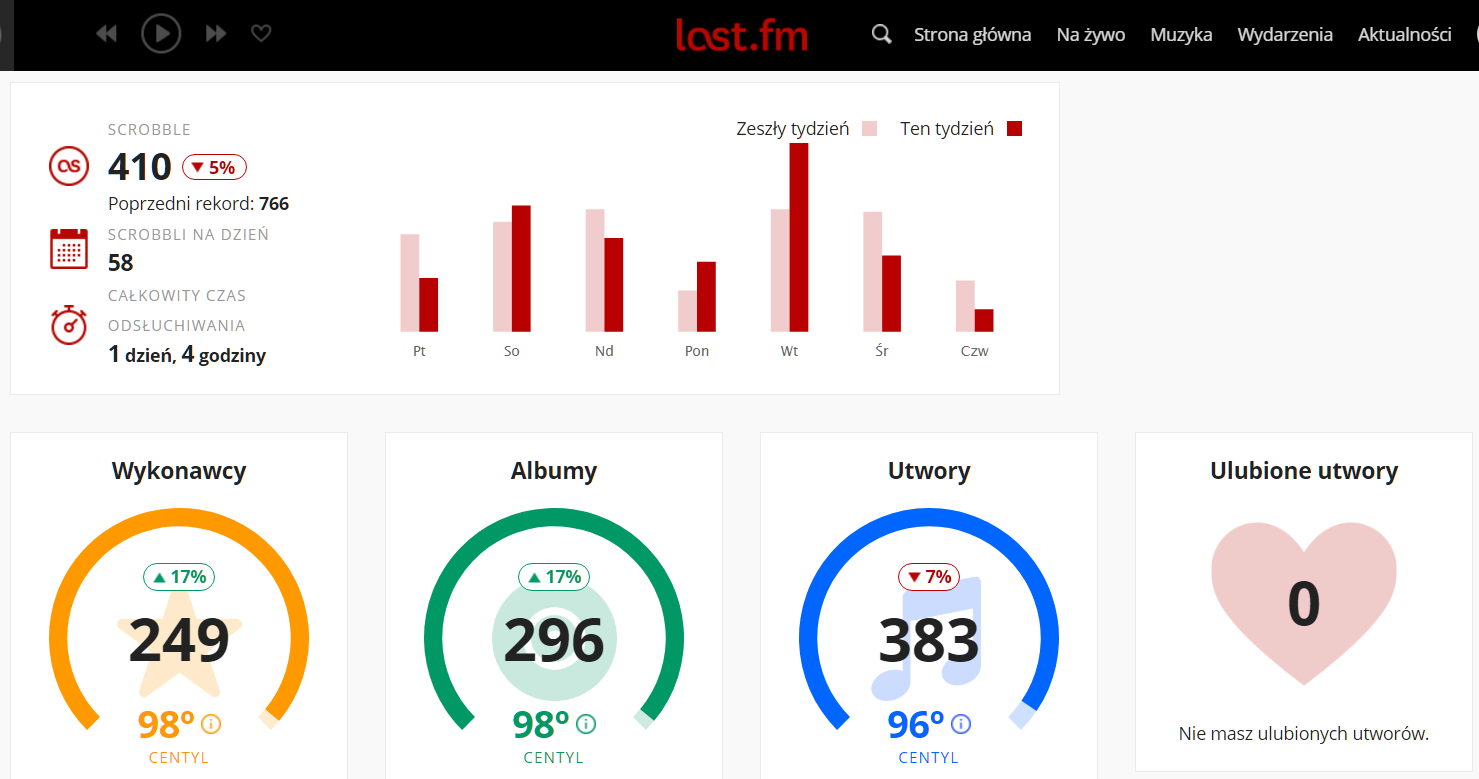
\includegraphics[width=\linewidth]{fig/lastfm-weekly.png}
                \caption{Tygodniowy raport słuchanej muzyki w Last.fm}
                \label{fig:lastfm-weekly}
            \end{figure}

            Last.fm to serwis społecznościowy pomagający odkrywać nowych artystów na podstawie poprzednich odsłuchów użytkownika.

            Wtyczka "Last.fm Scrobbler" \cite{lastfm:trackmymusic} integruje się z odtwarzaczami muzycznymi, np. Spotify.
            Każdy odsłuchany w co najmniej w połowie utwór jest logowany do bazy danych,
            w której na podstawie ID3 tagów jest przypisywany do artysty, płyty oraz gatunku muzycznego.

            Serwis udostępnia szereg metod REST API \cite{lastfm:apidoc}, dla mnie szczególnie istotne są te
            związane z odtworzeniami użytkownika oraz szczegółowych informacji o piosenkach i artystach.

            Szczegółowe informacje są dostępne po podaniu ich MBID\cite{lastfm:mbid} lub nazwy (piosenki lub artysty).
            Pierwszy sposób jest preferowany, choć nie zawsze dostępny. Gwarantuje unikalność identyfikatora oraz uniknięcie problemów kodowania znaków.

    \section{Mechanizm importu danych}
        Przed analizą, konieczne jest pobranie danych do własnej bazy danych oraz stworzenie modelu relacji pomiędzy nimi.
        Proces pobierania nazywam agregacją danych lub importem danych i jest on podstawą działania aplikacji,
        ponieważ to w nim zdobywamy interesujące nas informacje wykorzystywane do późniejszych obliczeń.

        Aby aplikacja nie była jednorazowego użytku, wraz z upływem czasu należy dla każdego użytkownika dostarczać
        kolejne porcje danych z zewnętrznych serwisów.
        Rodzi to szereg problemów oraz wyznacza pewne cechy, które implementacja powinna spełniać.

        \subsection*{Niezależność}
            Podczas pobierania danych dla jednego użytkownika może wystąpić błąd, np. poprzez tymczasową niedostępność API,
            nie powinien on wpłynąć na agregacje innych użytkowników, ani na działanie mechanizmu w przyszłości dla tego samego użytkownika.

            Części błędów można się spodziewać, np. Last.fm udostępnia do każdej metody API listę błędów, które może zwrócić zamiast odpowiedzi.
            Z drugiej strony, mogą wystąpić błędy po naszej stronie --- zwłaszcza gdy API nie jest bardzo dobrze udokumentowane
            lub nie mamy zbyt dużego doświadczenia z pracy z nimi, np. podczas mapowania odpowiedzi na obiekty lub przy zapisie danych do bazy.

            Można sobie z tym radzić na kilka sposobów, przechwytując wyjątki podczas wysyłania każdego requestu
            oraz dodatkowy error handler przechwytujący wszystkie wyjątki powstałe podczas budowania modelu i zapisywania danych w bazie,
            tak by błąd w agregacji jednego użytkownika nie wpływał na innych (oraz na jego następne).

            Dzięki kilku poziomom przechtywywania wyjątków, mamy możliwość decydowania o ich krytyczności.
            Nieudane requesty możemy dodawać do kolejki i po kilku minutach ponowić próbę ich wysłania.
            W przypadku błędu zapisu do bazy możemy zignorować jeden request lub oznaczyć całą aggregację do powtórzenia.

            Kolejkowanie requestow jest skuteczne, gdy API ma sztywny czas sesji np. 5 minut, po którym następuje wylogowanie.
            RescueTime i Last.fm mają autoryzację bezstanową,
            w pełni polegającej na raz wygenerowanym kluczu --- sesja nie jest tu problem,
            więc zdecydowałem się porzucić pomysł kolejkowania pojedynczych requestów.

        \subsection*{Ciągłość}

            \begin{figure}
                \centering
                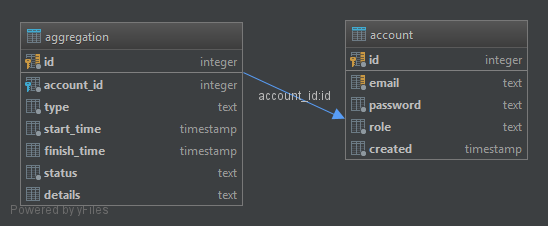
\includegraphics[width=\textwidth]{fig/db-aggregation.png}
                \caption{Schemat relacji aggregation}
                \label{fig:db-aggregation}
            \end{figure}

            Celem codzienne uruchamianie procedury i pobranie najnowszych lub brakujących danych do systemu,
            API pozwalają nam na wybranie tylko małego fragmentu danych, istotne jest więc by zacząć import
            od momentu ostatniego poprawnie wczytanego rekordu dla danego użytkownika.

            Podczas pierwszej agregacji, domyślnie pobierane są dane sprzed trzech miesięcy.
            Czas startu jest zapisywany do tabeli \mintinline{sql}|aggregation|,
            a każda następna aggregacja będzie zaczynała się od momentu skończenia poprzedniej.

            W przypadku niepowodzenia, błąd zapisywany jest w bazie danych - ale nie wpływa na kolejne agregacje,
            takie rekordy mają charakter informacyjny dla developera i są ignorowane w późniejszych agregacjach.

            Pobrane rekordy nie są bezpośrednio połączone z konkretną agregacją,
            chcąc się dowiedzieć jakie rekordy były pobrane, należy pobrać wszystkie rekordy pomiędzy datą konkretnej agregacji oraz poprzedzającej ją.

            Na poziomie aplikacji, regularne odpalanie procedury importu zajmuje się klasa \mintinline{java}{AggregationScheduler}
            która korzysta z Spring Schedulera i CRONa, codziennie o 3 w nocy puszcza agregacje dla użytkowników z poprawnie wypełnioną konfiguracją.

        \subsection*{Powtarzalność}

            Ważna jest możliwość uruchomienia fragmentu kodu niezależnie od całości agregacji, np. chcąc sprawdzić połączenie API z konkretnymi parametrami
            lub uruchomić tylko fragment mapowania odpowiedzi na bazodanowe encje.
            Dzięki temu, w przypadku problemów jesteśmy w stanie przeanalizować działanie od wybranego przez nas momentu,
            bez uruchamiania całej 20-minutowej procedury.

            Podczas pisania pierwszej wersji programu w NodeJS, zignorowałem ten aspekt co poskutkowało czasochłonną analizą błędów,
            a w ostateczności przepisaniem kodu.

            % TODO: Wspomnieć o TDD

    \section{Komunikacja z API}

        \subsection*{Specyfika odpowiedzi API}
            Przy projektowaniu rozwiązania warto pamiętać o tym, że nie istnieje powszechnie wykorzystywany standard budowania API,
            a każdy dostawca implementuje je w sposób specyficzny dla swojego systemu i danych, jakie udostępnia.

            RescueTime, mimo że co do sekundy loguje start i koniec aktywności,
            jego najwyższa dokładność oferowana użytkownikowi to 5 minut \footnote{TODO: rescuetime:apidoc-precision},
            a w darmowej wersji zezwala na dostęp maksymalnie trzy miesiące wstecz.

            RescueTime oferuje jeden, mocno konfigurowalny endpoint, który obsługuje wszystkie zapytania.
            Struktura odpowiedzi również jest bardzo generyczna, przypominająca CSV.
            W zależności od konfiguracji, zmieniają się nagłówki i schemat wierszy, należy napisać dodatkowy parser na własne API.

            \begin{minted}{java}
    @Data
    public class RescueTimeResponse {
        private String notes;
        private List<String> row_headers;
        private List<List<String>> rows;
    }
            \end{minted}

            Do bezpośredniej komunikacji stworzyłem klasę \mintinline{java}|RescueTimeCaller|, która buduje parametry requesta
            oraz przetwarza go za pomocą klienta ``Spring RestTemplate''. Zestaw testów jest w klasie \mintinline{java}|RescueTimeCallerTest|.

            \begin{minted}{java}
    public class PaginatedResult<T> implements Iterable<T> {
        private int page;
        private int totalPages;
        private Collection<T> pageResults;
    }
            \end{minted}

            W przypadku Last.fm, wynik odpowiedzi jest stronnicowany - jednym rządaniem możemy pobrać maksymalnie 100 utworów.
            Do wysyłania requestów i deserializacji odpowiedzi na obiekty
            wykorzystuję bibliotekę ``Last.fm API Bindings for Java''\cite{lastfm:java-bindings}.

            Schemat odpowiedzi XML w przypadku endpointów których używam jest taki sam, lecz w zależności od konfiguracji - różne pola są wypełniane.
            Przykładowo pole \verb|duration| zawierające długość piosenki jest puste, gdy używa się metody \verb|User.getRecentTracks|,
            a dostępne podczas używania metody \verb|Track.getInfo|.

        \subsection*{Autoryzacja}

        Do każdego requestu należy dodać klucze autoryzujące,
        które użytkownik musi wygenerować w serwisach Last.fm i RescueTime \cite{rescuetime:apidoc-keymanagment} oraz dodać w ustawieniach aplikacji.
        Klucze zapisywane są ws tabeli \textit{aggregation\_metadata}.
        Last.fm wymaga rejestracji aplikacji, po którym otrzymujesz dwa klucze: sekretny i normalny.

        W obu serwisach dostępne jest logowanie za pomocą OAuth, dzięki temu użytkownik nie musi samodzielnie generować kluczy,
        a jedynie potwierdzić chęć udostępnienia swoich danych w aplikacji. Zdecydowanie skraca i ułatwia proces konfiguracji.
        W obecnej wersji aplikacji nie używam tego mechanizmu, ale byłby on konieczny przed udostępnieniem jej publicznie.

        \begin{figure}
        	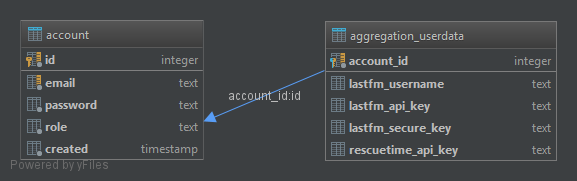
\includegraphics[width=\linewidth]{fig/db-aggregation-metadata.png}
        	\caption{Schemat relacji aggregation\_metadata}
        	\label{fig:db-aggregation-metadata}
        \end{figure}

        \subsection*{Niepełne dane}
        API mimo starań dostawców, może zawierać nieścisłości i luki informacji.
        Last.fm do identyfikacji utworu dostarcza jego MBID oraz pełną nazwę.
        Bezpieczniej jest korzystać z identyfikatora mbid, ponieważ w nazwie mogą występować problematyczne znaki UTF-8 np. w przypadku Chińskich artystów.
        Niekiedy nie jest to możliwe, istnieją bowiem rekordy, dla których identyfikator jest pusty.

        W przypadku braku MBID jest możliwe,
        że tytuł utworu zawiera zbyt dużo informacji (np. oznaczenie wersji koncertowej lub radiowej),
        lub utwór jest zbyt świeży. W takich przypadkach często brakuje informacji o długości takich piosenek.
        W bazie danych mam 505 takich utworów (21\% wszystkich).

        W danych RescueTime odnalazłem, że wyjątkowo dużo zadań jest przypisanych do akcji ``Google Chrome''.
        Według idei tego seriwsu wszystkie strony powinny mieć swoje akcje. Sugeruje to błąd podczas sczytywania przez program.
        Problem jest znany i opisany na stronie z pomocą \cite{rescuetime:help-browser-time}.

        \subsection*{Wydajność}
        Agregacja jest czasochłonnym procesem, nie ma powodu by dwa razy pobierać te same dane.
        Dobrą praktyką jest kopiowanie wszystkich pobranych informacji do własnej bazy danych,
        dzięki temu możemy ograniczyć ilość żądań do API tylko do nieznanych nam obiektów i zmniejszyć ryzyko wyczerpania limitu requestów.

		Żądania są wysyłane synchronicznie, jeden po drugim.
		Przy skali tysięcy requestów i średnim czasie requestu wahającym się między pół a dwiema sekundami, jest to istotna optymalizacja.
		Przeprowadziłem test dla danych z 90 dni Last.fm. Do pobrania 5992 rekordów, należało wysłać 60 requestów (60 stron) i trwało to około minuty.
		Dla każdego z nich należy pobrać dodatkowe szczegóły, co trwa około 26 minut.

		Wiele z tych 5992 rekordów się powtarza, dlatego po zapamiętaniu powtarzających się rekordów --- pełna agregacja trwa 13 minut.
		Im więcej rekordów w bazie, tym mniej żądań potrzeba wysłać i czas importu będzie coraz krótszy dla kolejnych użytkowników.

\chapter{Analiza danych}

	Po pojawieniu się pierwszych danych można zacząć je przeszukiwać i eksperymentalnie łączyć między sobą.
	Zacznę od zobrazowania skali danych, po jakiej się poruszam.
	Zaimportowane dane są z okresu od 31 stycznia do 4 maja 2017 z aktywności wykonywanych na prywatnym laptopie
	oraz od 3 lutego do 4 maja 2017 ze słuchanej muzyki z wielu urządzeń i komputerów.

	W tym 3-miesięcznym okresie wykonałem 34611 akcji, które są przypisane do 1916 programów lub stron internetowych z podziałem na 62 kategorie.
	Łącznie 588 godzin w ciągu 94 dni, średnio 6.2 godziny dziennie.
	Z czego 60.5\% to aktywności oznaczone jako produktywne, a 39.5\% jako rozpraszające lub neutralne.

	W ciągu 91 przeanalizowanych dni przesłuchałem 395 godzin muzyki — średnio 4.3 godziny dziennie.
	Składa się na to 5203 odtworzeń piosenek, z czego 2303 unikalnych wśród 1155 artystów.
	Odsłuchane piosenki były przypisane przez społeczność Last.fm do 1185 różnych tagów — najpopularniejsze z nich to: rock, polish, soundtrack
	(przyporządkowane odpowiednio do 543, 423, 347 piosenek).

	Warto już na początku zwrócić uwagę na długość pojedynczych akcji, 38\% ze wszystkich pojedynczych akcji trwało poniżej 10 sekund.
    % TODO: 19 sekund czy 5? Decyzja.
	Duża część z nich była szybkim wyszukiwaniem w Google lub w ogóle nieskategoryzowana.
	Natomiast zaledwie 17\% akcji trwało ponad 2 minuty, w tym przypadku częstszą kategorią są rzeczy związane z programowaniem oraz grami.

	    \begin{table}[]
        \centering
        \begin{tabular}{|l|l|l|}
            \hline
            Kategoria                           & Ilość zadań (x)   & \%      \\ \hline
            \multicolumn{2}{|c|}{Zadania trwające poniżej 5 sekund} & x / 6784\\ \hline
            Browsers                            & 1040              & 15.3\%  \\ \hline
            General Utilities                   & 755               & 11.1\%  \\ \hline
            GeneralSocial Networking            & 564               & 8.3\%   \\ \hline
            Search                              & 563               & 8.2\%   \\ \hline
            Uncategorized                       & 551               & 8.1\%   \\ \hline
            \multicolumn{2}{|c|}{Zadania trwające ponad 2 minuty}   & x / 5012\\ \hline
            Browsers                            & 1047              & 20.8\%  \\ \hline
            Editing \& IDEs                     & 821               & 16.3\%  \\ \hline
            General Social Networking           & 570               & 11.3\%  \\ \hline
            General Software Development        & 408               & 8.1\%   \\ \hline
            Games                               & 282               & 5.6\%   \\ \hline
        \end{tabular}
        \caption{Lista najpopularniejszych kategorii wśród krótkich zadań poniżej 5 sekund oraz tych powyżej 2 minut}
        \label{Zadania krótkie i długie, które są najpopularniejsze?}
        \end{table}

\section{Opis zebranych danych}

    \subsection*{RescueTime --- aktywności}
    \begin{figure}
        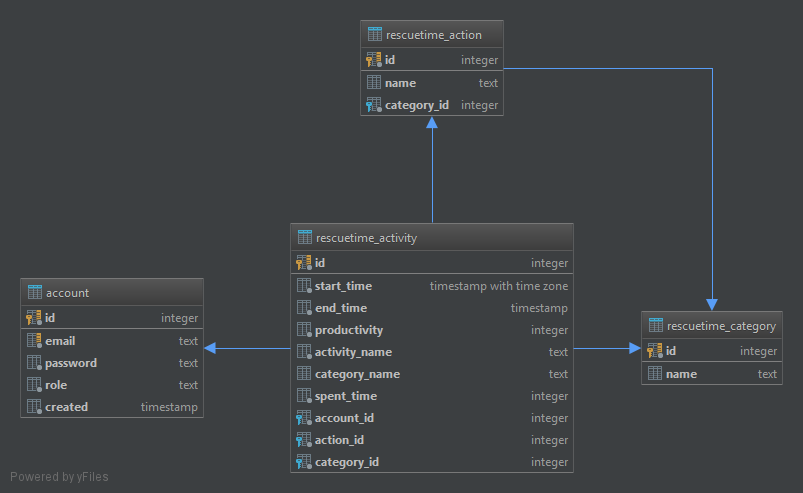
\includegraphics[width=\linewidth]{fig/db-rescuetime-schema.png}
        \caption{Schemat relacji danych o aktywnościach}
        \label{fig:db-rescuetime-schema}
    \end{figure}

    Najważniejszą tabelą wśród tych powiązanych z aktywnościami jest \verb|rescuetime_activity|,
    to do niej w pierwszej kolejności trafiają dane z API bez żadnej obróbki,
    następnie nazwa akcji oraz kategoria są przyporządkowywane do istniejących rekordów w tabelach
    \verb|rescuetime_action|, oraz \verb|rescuetime_category| lub utworzone nowe w razie konieczności.
    Ma to na celu wygodniejsze przygotowanie danych i wykresów na podstawie konkretnej kategorii
    oraz ograniczenie nadmiarowości danych w przyszłości.

    \begin{table}
    \centering
    \begin{tabular}{|l|l|l|}
        \hline
        kolumna             & Rekord 1             & Rekord 2           \\ \hline
        \verb|id|           & 14226                & 14251              \\
        \verb|account_id|   & 1                    & 1                  \\ \hline
        \verb|start_time|   & 2017-01-31 09:20:00  & 2017-01-31 10:05:00\\
        \verb|end_time|     & 2017-01-31 09:25:00  & 2017-01-31 10:10:00\\ \hline
        \verb|productivity| & +2                   & -2                 \\
        \verb|spent_time|   & 4s                   & 12                 \\ \hline
        \verb|action_id|    & 138                  & 22                 \\
        \verb|activity_name|& evernote.com         & spotify            \\ \hline
        \verb|category_id|  & 17                   & 34                 \\
        \verb|category_name|& Writing              & Music              \\ \hline
    \end{tabular}
        \caption{Przykładowy rekord z tabeli rescuetime\_activity}
        \label{RescueTime --- Przykładowy rekord z tabeli rescuetime_activity}
    \end{table}

    \subsection*{Last.fm --- Muzyka}

    \begin{figure}
        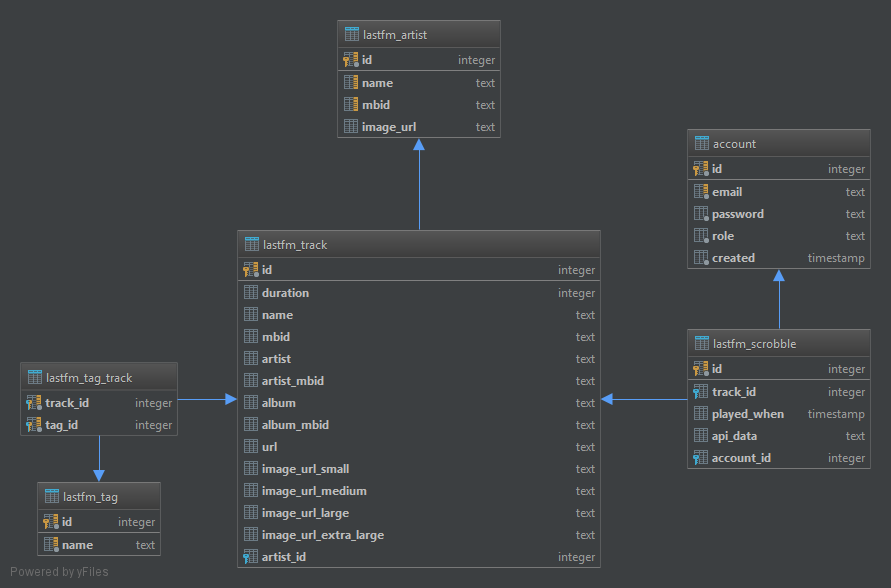
\includegraphics[width=\linewidth]{fig/db-lastfm-schema.png}
        \caption{Schemat relacji danych o muzyce}
        \label{fig:db-lastfm-schema}
    \end{figure}

    Dane muzyczne są dużo bardziej rozproszone od aktywności, zapisuje je do 5 połączonych tabel.
    Jej sercem jest tabela \verb|lastfm_scrobble|, przechowująca każde pojedynczy odsłuch piosenki przez użytkownika.
    Zawiera ono moment startu odsłuchu oraz jest punktem startowym do pozostałych relacji (poprzez tabelę \verb|lastfm_track|).
    Ważnym polem jest \verb|api_data| w którym zapisuję wszystkie zwrócone dane z API w czystej postaci dla danego scrobbla (rekordu).
    Pomaga ono przy debugowaniu mapowań pomiędzy API a opisywanym serwisem.

    \section{Korekta}

        Dane zapisywane są w 5-minutowych okienkach ze względu na ograniczenia API, to dobry moment na sprawdzenie duplikatów.
        Suma wszystkich aktywności w każdym oknie nie powinna przekroczyć 300 sekund.
        Okazuje się, że w 1337 5-minutowych okresach, istniały duplikaty.
        Nie jest określone czy pochodzą one bezpośrednio z API, czy z powodu błędu w kodzie.

        Postanowiłem je omijać w momencie generowania danych, bazując na trzech unikalnych polach:
        \verb|DISTINCT ON (start_time, activity_name, spent_time)|.
        Możliwe jest, że tą metodą usuniemy również aktywności, które w rzeczywistości nie byłyby duplikatami,
        prawdopodobieństwo jest wysokie przy czynnościach trwających bardzo krótko np. dwa razy otwarta wyszukiwarka na 3 sekundy.
        Jest to akceptowalne ryzyko błędu, jako że bardzo krótkie aktywności mają mniejsze znaczenie dla dalszej analizy.

        Dane utworów z Last.fm często nie zawierają informacji o długości piosenki.
        Brakuje ich, gdy nazwa jest niestandardowa lub gdy artysta jest niszowy i dane nie zostały uzupełnione przez społeczność Last.fm.
        Zorientowałem się o tym podczas budowania wykresu najpopularniejszych artystów,
        kiedy artysta ``Scott BradLee's Postmodern Jukebox'' mając 33 odtworzenia, ma zarejestrowane zaledwie 9 minut odsłuchu.
        Zdecydowałem nadać im średnią długość ze wszystkich piosenek przesłuchanych przez użytkownika.
        W moim przypadku średnia wynosi 232 sekundy (liczone tylko z piosenek o długości dłuższej od zera).

    \section{Integracja źródeł danych}

        Najważniejszym elementem tej pracy jest połączenie obu źródeł danych,
        dopiero na tej podstawie możemy wysnuć tytułowy wpływ muzyki na aktywności wykonywane przy komputerze.

        Jeżeli chodzi o muzykę, muzyka słuchana poza komputerem jest dla nas nieinteresująca,
        dlatego punktem wyjścia jest lista aktywności i to do każdej z nich będziemy dopasowywać muzykę. Nie na odwrót.
        Z drugiej strony nie chcemy ignorować aktywności, które były wykonywane w ciszy.
        Dane wymagania doprowadzają nas do poniższego zapytania SQL (uproszczonego dla przykładu):

\begin{minted}{sql}
SELECT *
  FROM rescuetime_activity activity
    LEFT JOIN lastfm_scrobble scrobble
      ON scrobble.played_when >= activity.start_time
         AND scrobble.played_when <= activity.end_time
         AND scrobble.account_id = activity.account_id
  ORDER BY played_when DESC;
\end{minted}

        Warto zaznaczyć, że zapytanie napisane w ten sposób duplikuje dane aktywności,
        jeżeli podczas ich wykonywania będzie odsłuchiwana więcej niż jedna piosenka.

        Łączenie tabeli za pomocą porównań dat jest bardzo niewydajne,
        powyższe zapytanie wykonuje się około 5 minut dla danych jednego użytkownika z około 3 miesięcy.
        Taki czas jest niedopuszczalny.

        Jednym z rozwiązań jest stworzenie widoku w PostgreSQL typu \verb|MATERIALIZED|.
        SQL wykonuje się tylko podczas tworzenia widoku, a rezultat zostaje jako tymczasowa tabela.
        Każde wywołanie danych widoku w tym przypadku kosztuje bardzo mało --- tyle samo co pobranie danych ze zwykłej tabeli.
        Dane w tej tymczasowej tabeli nie zmienią się, dopóki ręcznie nie zostanie ręcznie odświeżony komendą
        \verb|REFRESH MATERIALIZED VIEW xyz|. Jest to rozsądne rozwiązanie, gdy dane rzadko się zmieniają, a ich pobranie jest kosztowne.

        Nie rozwiązuje to jednak problemu inicjalnego czasu działania tego zapytania,
        5 minut to wciąż dużo --- nawet gdyby wykonywał się on raz dziennie w nocy.
        Rozwiązaniem długiego czasu łączenia jest nałożenie indeksów \cite{postgresql:efficient-indexes},
        nadanie ich na kolumny dat w tabeli \verb|rescuetime_activity| przyspiesza zapytanie do 1 minuty.
        Dodanie indeksów na tabeli \verb|lastfm_scrobble| na kolumnę \verb|played_when| powoduje czas wykonania poniżej 300ms.

\begin{minted}{sql}
CREATE INDEX rescuetime_activity_start_end_time_index
  ON rescuetime_activity (start_time, end_time);
CREATE INDEX lastfm_scrobble_played_when_index
  ON lastfm_scrobble (played_when);
\end{minted}

\chapter{Wizualizacja danych}

    Produktem dla końcowego użytkownika jest aplikacja webowa, która podsumowuje zebrane wcześniej dane.
    Jest ona oparta na klasycznym podejściu MVC z kilkoma podstronami z częścią dynamicznych komponentów.

    Jeden zbiór danych może mieć wiele interpretacji, przedstawione w tym rozdziale wykresy
    są efektem moich eksperymentów i poszukiwań, niekoniecznie obiektywnie odzwierciedlających rzeczywistość.

    \section{Budowa raportów na podstawie szeregów czasowych}

    Wyświetlane na raportach wykresy mogą mieć różną granularność w zależności od naszych potrzeb.

    \begin{minted}{sql}
    SELECT *
    FROM generate_series(
         date_trunc('day', :from ::TIMESTAMP),
         date_trunc('day', :to ::TIMESTAMP),
         '1 day' :: INTERVAL
     ) date
    \end{minted}

    Powyższy przykład generuje zbiór dat z jednodniowym interwałem,
    który możemy połączyć z innymi tabelami za pomocą \mintinline{sql}|LEFT JOIN|.
    Dzięki teumu mamy pewność, że ilość rekordów będzie zawsze stała i niezależna od danych z innych tabel.
    Nawet w przypadku gdy dla danej daty, nie ma żadnych odpowiedników - rekord z datą będzie widoczny.

    Funkcja \mintinline{sql}{generate_series(start, stop, step)} tworzy zbiór elementów
    zaczynających się od pierwszego argumentu do drugiego z zadanym interwałem.
    Funkcja \mintinline{sql}|date_trunc(precision, timestamp)| ucina datę do zadanej precyzji.
    \mintinline{sql}|date_trunc('hour', timestamp '2017-05-01 23:38:40')| zwraca \\ \mintinline{sql}|2017-05-01 23:00:00|

    Zakres dat podawany jest w parametrze \mintinline{sql}|:from| i \mintinline{sql}|:to|,
    jest generowany przez serwis w zależności od potrzeb raportu.
    Dla metody zwracającej raport z całego miesiąca, oblicza się pierwszy i ostatni jego dzień.

    \begin{minted}{java}
List<ArtistsSummary> mostPopularArtists(
        int year, int month, long accountId) {
    LocalDate firstDayOfMonth = LocalDate.of(year, month, 1);
    LocalDate lastDayOfMonth = firstDayOfMonth.withDayOfMonth(
        firstDayOfMonth.lengthOfMonth()
    );

    return artistsRepository.mostPopularArtists(
        firstDayOfMonth, lastDayOfMonth, accountId
    );
}
    \end{minted}

    \begin{figure}
        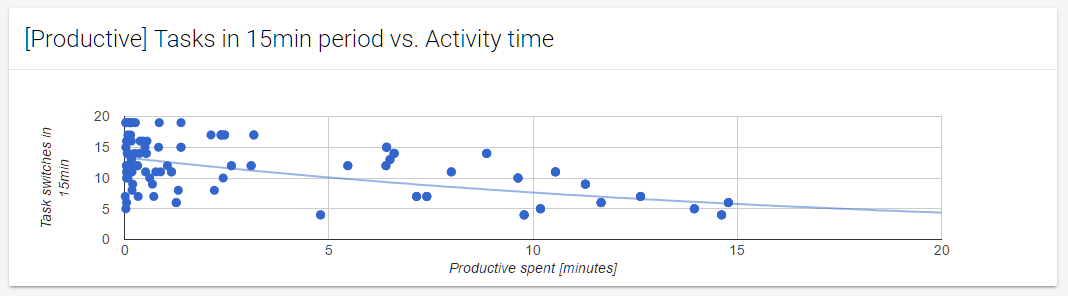
\includegraphics[width=\linewidth]{fig/ui/chart-tasks-productive.png}
        \caption{Wykres: Wpływ ilości zadań w ciągu 15minut na długość produktywnych zadań}
        \label{fig:ui:chart-tasks-productive}
    \end{figure}

    \begin{figure}
        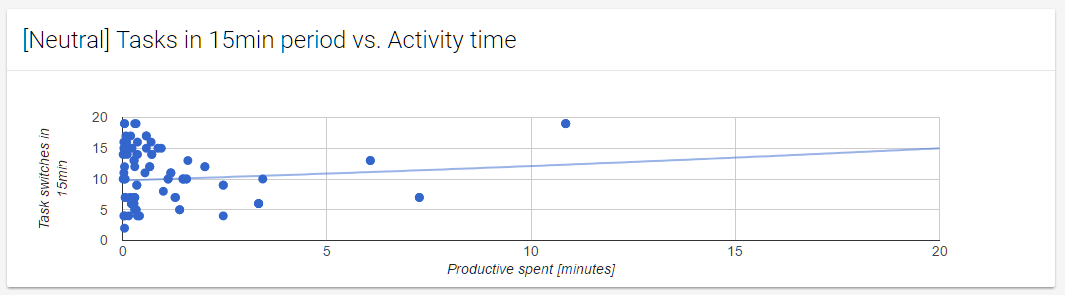
\includegraphics[width=\linewidth]{fig/ui/chart-tasks-neutral.png}
        \caption{Wykres: Wpływ ilości zadań w ciągu 15minut na długość neutralnych zadań}
        \label{fig:ui:chart-tasks-neutral}
    \end{figure}

    \begin{figure}
        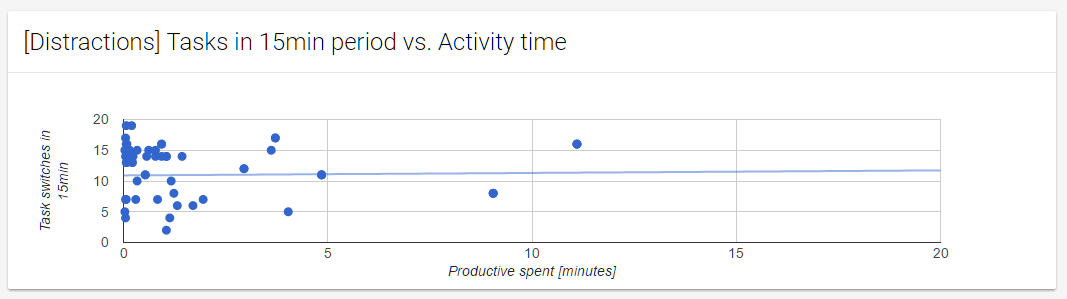
\includegraphics[width=\linewidth]{fig/ui/chart-tasks-distractions.png}
        \caption{Wykres: Wpływ ilości zadań w ciągu 15minut na długość rozpraszających zadań}
        \label{fig:ui:chart-tasks-distractions}
    \end{figure}

    \begin{figure}
        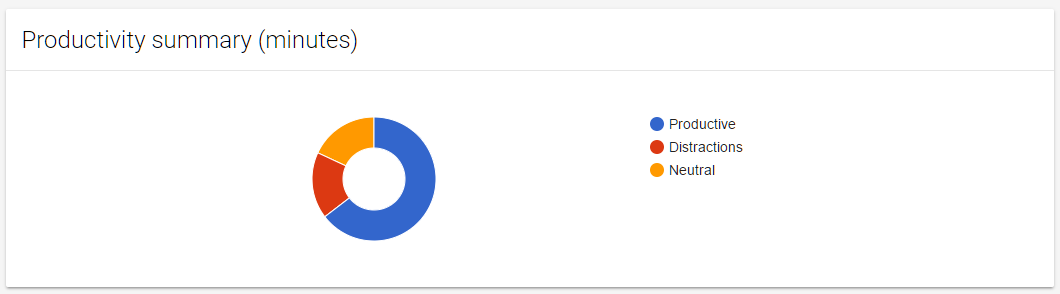
\includegraphics[width=\linewidth]{fig/ui/chart-productivity-summary.png}
        \caption{Wykres kołowy: }
        \label{fig:ui:chart-productivity-summary}
    \end{figure}

    \section{Wiarygodność}

    Zanim przystąpi się do wyciągnięcia wniosków, należy sprawdzić czy dane w systemie są wiarygodne.

    \begin{figure}
        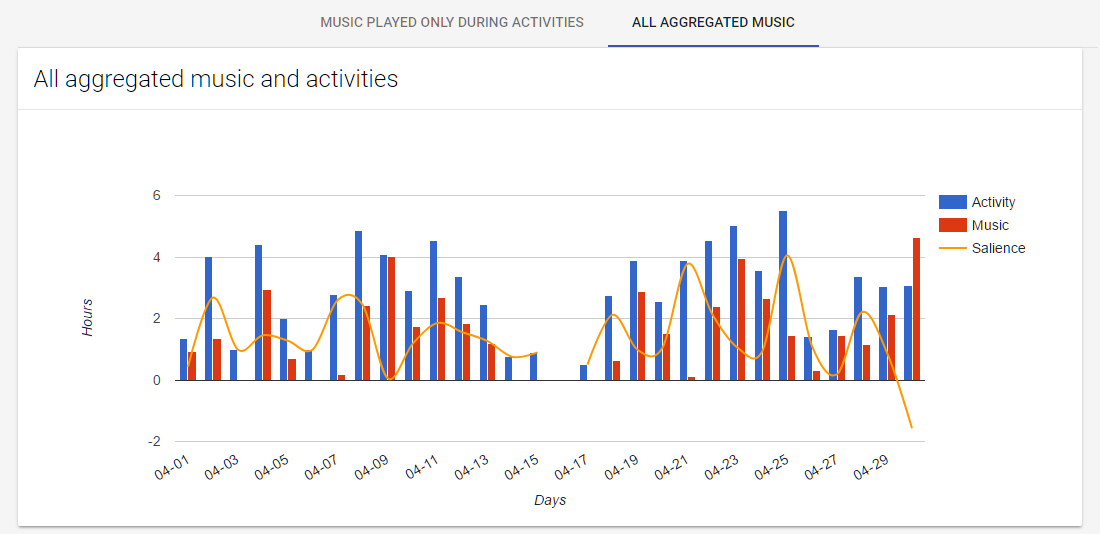
\includegraphics[width=\linewidth]{fig/ui/chart-music-all.png}
        \caption{Wykres: Dzienna długość wykonywanych aktywności i przesłuchanej muzyki (czas trwania muzyki może być większy od aktywności)}
        \label{fig:ui:chart-music-all}
    \end{figure}

    \begin{figure}
        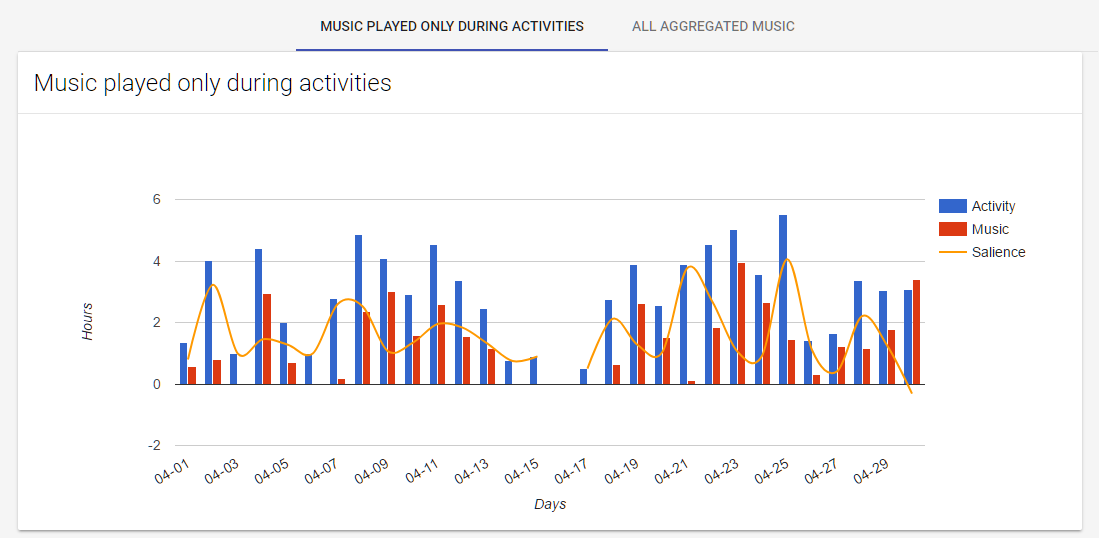
\includegraphics[width=\linewidth]{fig/ui/chart-music-only-during-activities.png}
        \caption{Wykres: Dzienna długość przesłuchanej muzyki tylko podczas wykonywanych aktywności na laptopie}
        \label{fig:ui:chart-music-only-during-activities}
    \end{figure}

    \section{Wybór metod wizualizacji danych}

    Wizualna reprezentacja pozwala na lepsze zrozumienie genezy danych, skategoryzować je i znaleźć korelację.
    Można wykrywać nieprawidłowości oraz starać się definiować trendy, wiele zależy od interpretacji i intencji analityka.
    \cite{charts:excel-comparsion}

    W aplikacji, do reprezentacji danych użyłem kilku powszechnie stosowanych typów wykresów.
    Tabele służą mi do pokazania niedużej liczby danych w określonym porządku,
    np. lista najpopularniejszych artystów lub tagów ze zdjęcia \ref{fig:ui:table-popular-music-tags}.
    Wyłania to najważniejszych przedstawicieli danych, omijając potencjalnie długą listę rekordów.

    \begin{figure}
        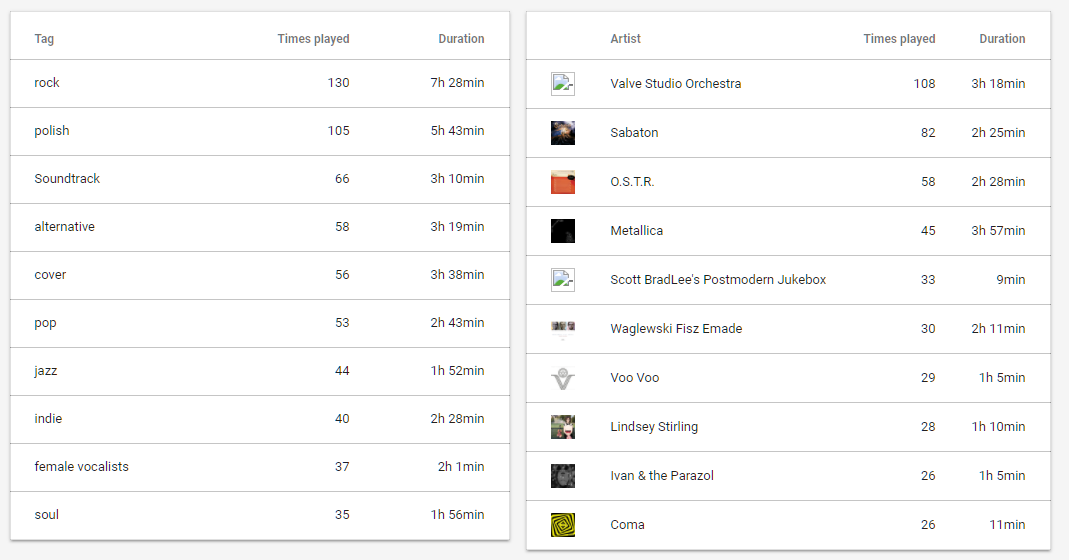
\includegraphics[width=\linewidth]{fig/ui/table-popular-music-tags.png}
        \caption{Tabela z najpopularniejszymi tagami i artystami w miesiącu w raz z łączną długością odtworzeń. Screenshot z aplikacji.}
        \label{fig:ui:table-popular-music-tags}
    \end{figure}

    Wykresy łączone, jak te pokazane na rysunku \ref{fig:ui:chart-music-all} i \ref{fig:ui:chart-music-only-during-activities},
    użyłem w celu wyróżnienia jednej kategorii (czasu ciszy) i podkreślenia jej stosunku wobec dwóch pozostałych (czasu aktywności oraz słuchania muzyki).
    Na pierwszym wyrkesie \ref{fig:ui:chart-music-all} wskazuje również nieprawidłowość jaką jest ujemny czas ciszy,
    który występuje gdy słuchamy na urządzeniach innych niż na których pracujemy.

\chapter{Architektura}

    \begin{figure}
        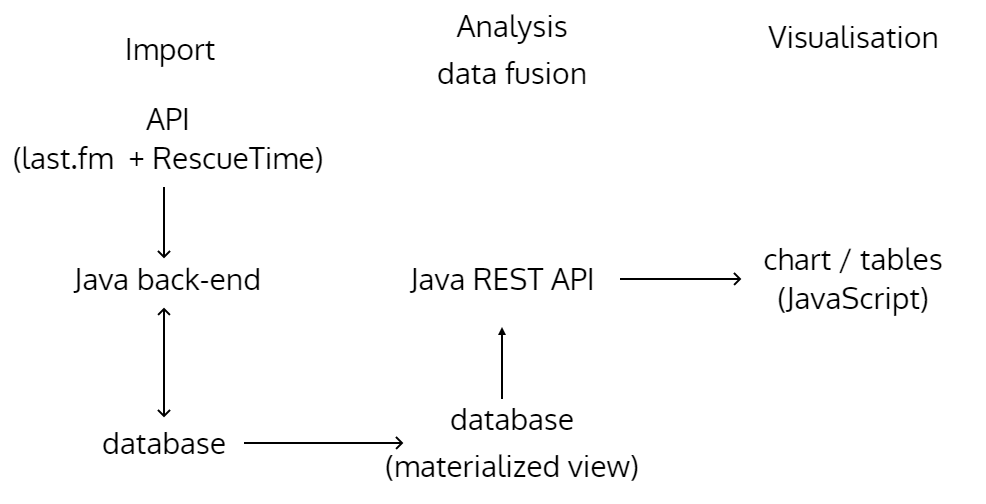
\includegraphics[width=\linewidth]{fig/data-flow.png}
        \caption{Przepływ danych w aplikacji podzielony na części importu, analizy i wizualizacji}
        \label{fig:data-flow}
    \end{figure}

    Do uruchomienia projektu wymagana jest Java 8 JRE oraz zainstalowany PostgreSQL.
    Pobraniem zależności i zbudowaniem paczki zajmuje się komenda \mintinline{bash}|./gradlew build|,
    wygenerowany WAR można osadzić na serwerze aplikacji Tomcat lub uruchomić komendą \mintinline{bash}|java -jar file.war|,
    wówczas uruchomi się wbudowany w aplikację serwer ``Embedded tomcat''.

    Z każdą zmianą w bazie danych, należy stworzyć nowy plik migracji SQL oraz uruchomić.
    Obecne są przechowywane w katalogu projektu: \mintinline{bash}|/main/resources/migration/|

    Projekt dzieli się na trzy główne części.
    - Import danych do bazy, jest to główne źródło pozyskiwania danych, komunikacji z API.
    - REST API - przeznaczone do wybierania już przetworzonych danych w postaci przyjaznej dla front-endu
    - MVC - Aplikacja bezpośrednio widoczna dla użytkownika, zawiera prosty back-end oraz front-end który komunikuje się z REST API.
    Obsługuje mechanizm autentykacji.

    %TODO - wspomnieć o migracjach sql
    %TODO - rozrysować przepływ danych jako sekcja
    %TODO - opisać strukturę paczek (opcjonalne)

\section{Testy jednostkowe}

Część kodu była napisana metodologią TDD,
kod API zwracającego przeanalizowane dane nie jest przetestowany głównie dlatego,
że główna logika jest w tym przypadku w zapytaniach SQL.

Code coverage dla całego projektu wygląda tak:
\begin{table}

	\begin{tabular}{|r|c|c|c|}
		\hline
		Moduł & Pokrycie klas & Pokrycie metod & Pokrycie operacji \\ \hline
		Średnia projektu & 75\% (58 na 77) & 42\% (159 na 378) & 53\% (473 na 891) \\
		Moduł agregacji & 94\% (37 na 39) & 61\% (134 na 219) & 73\% (385 na 521) \\
		API & 43\% (10 na 23) & 8\% (10 na 122) & 12\% (35 na 270) \\  \hline
	\end{tabular}

    \caption{
	Code coverage projektu Java
	}
\label{Projekt --- Code coverage}
\end{table}

\section{Narzędzia}

    Projekt zrealizowano dzięki wielu projekom open-source, w tej sekcji listuję najważniejsze z nich.

%TODO: Licencja
\begin{table}
\begin{tabular}{|l|c|l|}
	\hline
	Nazwa narzędzia & Wersja & Opis zastosowania \\
	\hline
	Java & 8 & Główny język programowania \\
	\hline
	Spring Boot & 1.4 & Framework IoC + MVC + REST \\
    \hline
	Spring Security & TODO & Autoryzacja użytkowników \\
	\hline
	PostgreSQL & 9.6 & Silnik bazy danych \\
	\hline
	Thymeleaf & 3.0 & Silnik szablonów \\
	\hline
	u-mass:lastfm-java & 0.1.2 & Komunikacja z Last.fm API \\
	\hline
	GSON & 2.8 & Serializacja JSON \\
	\hline
	guava & 20.0 & Metody pomocnicze \\
	\hline
	Lombok & 1.16 & Java boilerplate-free code generator \\
	\hline
	Junit & TODO & Unit tests runner \\
	\hline
	Assertj & 3.5 & Biblioteka assercji testów \\
	\hline
    ECMAScript & 2016 & Renderowanie raportów \\
    \hline
    fetch API & - & Standard komunikacji HTTP w przeglądarce \\
    \hline
    Google Charts & TODO & Renderowanie wykresów \\
    \hline
\end{tabular}
    \caption{Code coverage projektu Java}
	\label{Projekt - Code coverage}
\end{table}

% zakończenie
\summary
[Work in progress]

% literatura (obowiązkowo):
\bibliographystyle{unsrt}
\bibliography{xml}

% spis tabel (jeżeli jest potrzebny):
\listoftables

% spis rysunków (jeżeli jest potrzebny):
\listoffigures

\oswiadczenie

\end{document}
